\documentclass[russian,11pt]{article}
\usepackage[russian]{babel}
\usepackage[utf8]{inputenc}
% Общие отступы для страницы
\usepackage[left=2cm,right=2cm,
    top=2cm,bottom=2cm,bindingoffset=0cm]{geometry}
% Работа с url
\usepackage{url}
% Работа с изображением
\usepackage{graphicx}
\usepackage{ragged2e}
\usepackage{float}
\graphicspath{ {./images/} }
% для листинга
\usepackage{listings}

%\usepackage{fontspec}
%\setmainfont{Times New Roman}
%\usepackage{amsmath}
%\usepackage{amsfonts}
%\usepackage{amssymb}


 
\makeatletter
\g@addto@macro\@floatboxreset\centering
\makeatother

\begin{document}
\title{Пишем свое первое расширение на Quarkus}
\author{Иванов Роман Александрович}

\maketitle

\newpage
\tableofcontents
\newpage

\section{Предисловие}
~

 Quarkus - это фреймворк, состоящий из ядра и набора расширений. Ядро основано на внедрении Context и Dependency Injection (CDI), а расширения обычно предназначены для интеграции сторонней инфраструктуры путем предоставления их основных компонентов в виде компонентов CDI.

\section{Что такое Quakus Extension}
\paragraph{	} Quarkus Extension- это просто модуль, который может работать поверх приложения Quarkus. Наиболее распространенный вариант использования такого расширения - запуск стороннего фреймворка поверх приложения Quarkus.

\section{Запуск приложения в простом java приложении}
\paragraph{ } 
Давайте попробуем реализовать расширение для отправки почты во время поднятия контекста приложения (будем его дальше называть notification). Но прежде чем мы углубимся, нам сначала нужно показать, как отправлять сообщения из основного метода Java. Это значительно облегчит реализацию расширения. Точкой входа для notification является API notification. Чтобы использовать это, нам нужен адрес отправителя и получателя:

\begin{figure}[H]
	\centering
	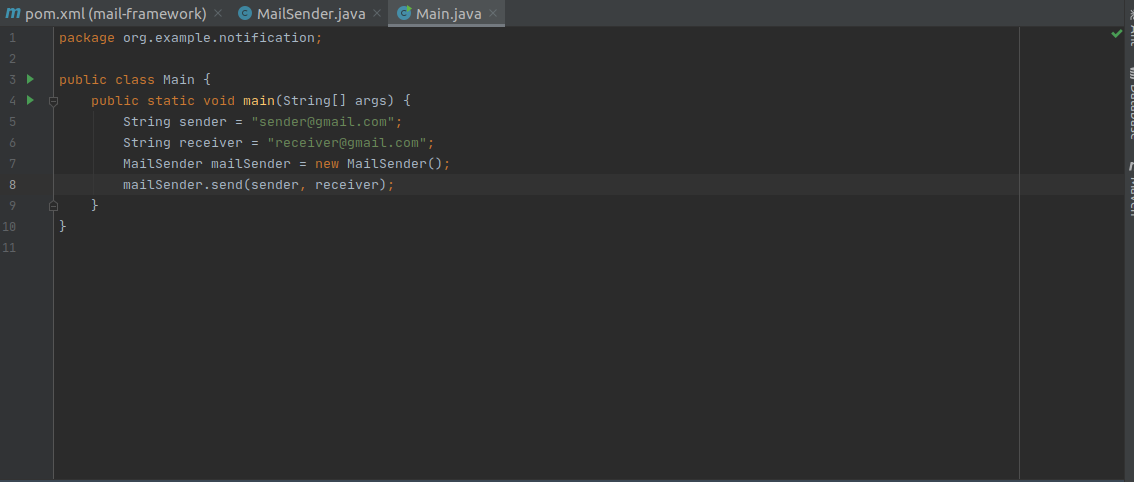
\includegraphics[scale=1.5, width=10cm]{1}
\end{figure}
~

При запуске можно увидеть следующее:

\paragraph{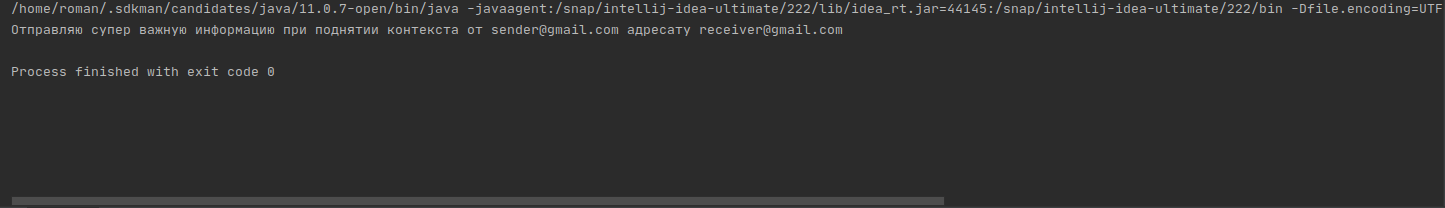
\includegraphics[scale=1.5, width=\textwidth]{2}}

~

Цель состоит в том, чтобы выставить notification как расширение Quarkus. То есть, предоставляя конфигурацию (адрес отправителя и получателя) Quarkus Configuration, а затем создавая notification  API в качестве компонента CDI. Это обеспечит средство для отправки сообщения в момент поднятия контекста приложения.

\section{Как создать расширение на простом примере}
~

Для ознакомления можно попробовать создать расширение самому, пройдя по ссылке \url{https://quarkus.io/guides/building-my-first-extension}. Все исходники по данной теме можно найти в архиве \textbf{firs-extention.zip}.
	
	Для того, чтобы создать расширение, необходимо выполнить инструкцию:

\lstinputlisting[language=sh]{latex-code/file.sh}

Обратите внимание, что указанная версия 1.4.2.Final является самой актуальной на момент написания, в зависимости от версии ее нужно будет поменять.

	Технически говоря, расширение Quarkus - это многомодульный проект Maven, состоящий из двух модулей. Первый - это модуль времени выполнения, в котором мы реализуем требования. Второй - это модуль развертывания для обработки конфигурации и генерации кода времени выполнения. Итак, начнем с создания многомодульного проекта Maven под названием quarkus-notification-parent, который содержит два подмодуля: время выполнения и развертывание:

\begin{figure}[H]
	\centering
	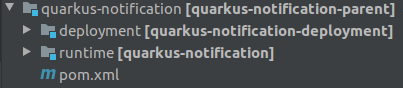
\includegraphics[scale=1, width=8cm]{3}
\end{figure}

\subsection{Имплементация runtime модуля}
\paragraph{ }
В runtime модуле мы реализуем:
 \begin{enumerate}
		\item[  1.] Конфигурационный класс, который будет хранить в себе настройки адресов отправителя и получателя)
		\item[  2.] Поставщика notification API (Предоставление расширением бина, который отвечает за notification API )
		\item[  3.] Рекордер, который будет работать как прокси обьект для вызова API
	\end{enumerate} 
	
	Модуль runtime будет зависеть от модуля ядра Quarkus и, в конечном итоге, модулей времени выполнения необходимых расширений. Здесь нам нужна зависимость нашей импровизированной библиотеки:

\begin{figure}[H]
	\centering
	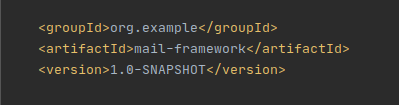
\includegraphics[scale=1.5, width=9cm]{4}
\end{figure}


После добавления этой зависимости в runtime модуль он будет выглядеть следующим образом:

\paragraph{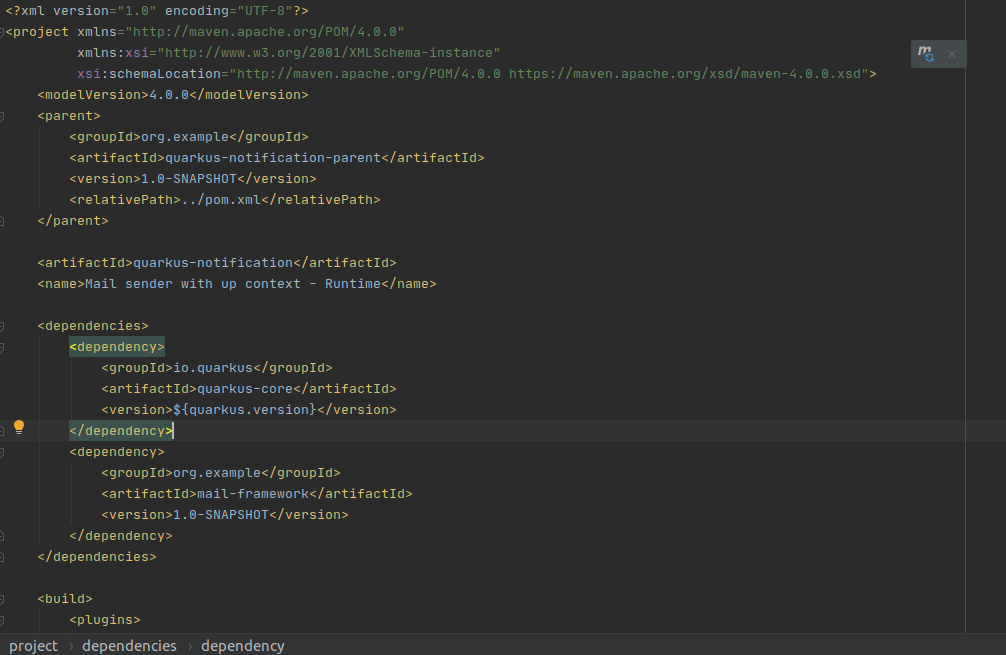
\includegraphics[scale=1.5, width=\textwidth]{5}}

\subsection{Реализация конфигурации}

Мы аннотируем класс с помощью @ConfigRoot, а свойства - с помощью @ConfigItem. Таким образом, поля from и to, будут представлены через ключ quarkus.mail.from и quarkus.mail.to в файле application.properties, расположенном в пути к классам приложения Quarkus.

	Также стоит обратить внимание на ConfigRoot.phase. Значение  BUILD\_AND\_RUN\_TIME\_FIXED означает, что значения ключей конфигурации читаются во время развертывания и доступен во время выполнения.
	
Конфигурационный класс будет иметь следующий вид:

\begin{figure}[H]
	\centering
	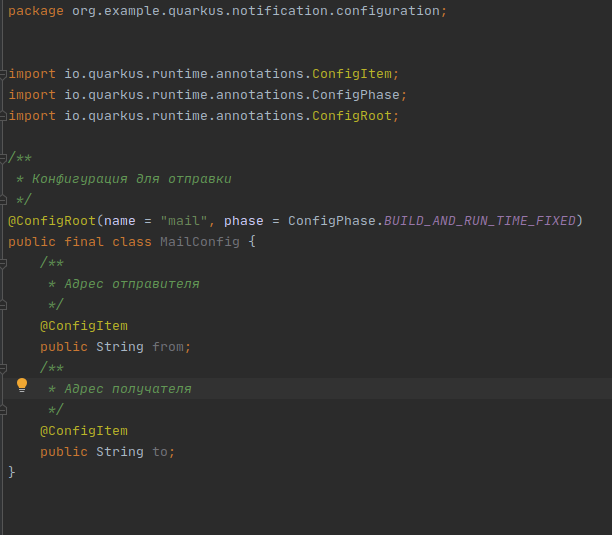
\includegraphics[scale=0.5, width=11cm, height=7cm]{6}
\end{figure}

\subsection{Имплементация поставщика notification API}

Выше мы видели, как работать с notification через простой вызов. Теперь мы воспроизведем тот же код, но в виде компонента CDI, и для этой цели будем использовать производителя CDI:

\begin{figure}[H]
	\centering
	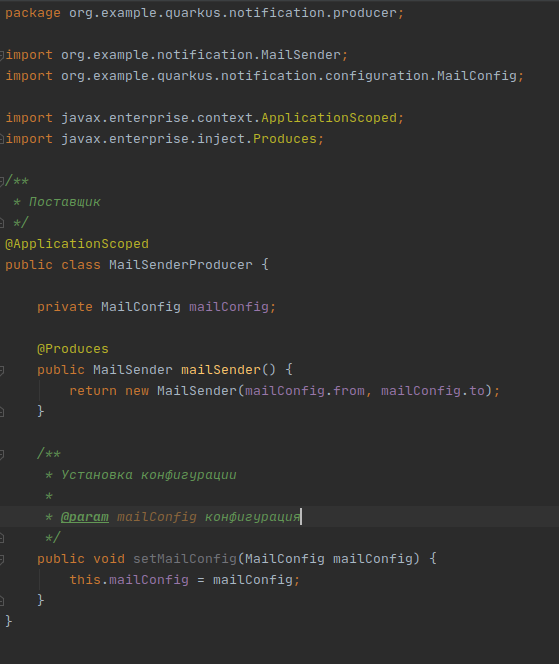
\includegraphics[scale=0.5, width=11cm]{7}
\end{figure}
	
	Метод, помеченный аннотацией @Produces, предоставляет бин с настройками, которые будут указаны в application.properties.

\subsection{Имплементация Рекордера}
~

На этом шаге мы напишем класс Рекордера, который действует как прокси для записи байт-кода и настройки логики времени выполнения:

\begin{figure}[H]
	\centering
	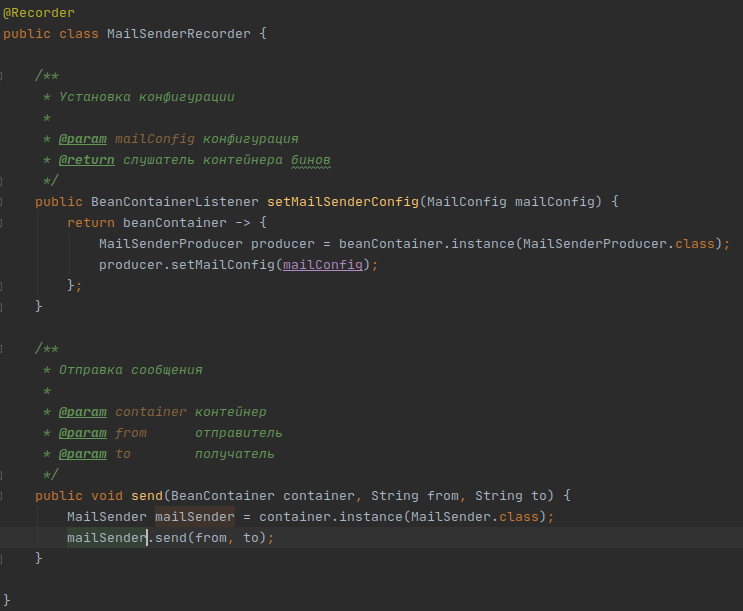
\includegraphics[width=13cm]{8}
\end{figure}
~

	Класс рекордер должен содержать аннотацию @Recorder. Через него мы устанавливаем конфигурацию, а также отправляем сообщение.
	
	Обратите внимание, что когда мы вызываем эти методы записи во время сборки, инструкции не выполняются, а записываются для последующего выполнения во время запуска.
	
Далее рассмотрим содержимое модуля развертывания (deployment).

\subsection{Реализация deployment}
~

Центральными компонентами расширения Quarkus являются процессоры Build Step. Это методы, аннотированные как @BuildStep, которые генерируют байт-код через устройства записи, и они выполняются во время сборки с помощью цели сборки модуля quarkus-maven-plugin, настроенного в приложении Quarkus.

	BuildSteps потребляют элементы сборки, созданные на ранних этапах сборки, и могут также сами создавать элементы сборки для других этапов сборки.

	Сгенерированный код всеми упорядоченными шагами сборки, найденными в модулях развертывания приложения, фактически является кодом времени выполнения.

\subsection{Сборка и настройка зависимостей}
~

Самым важным аспектом зависимостей данного модуля является то, что он должен зависеть от соответствующего модуля времени выполнения и, в конечном итоге, от модулей развертывания необходимых расширений. Это означает, что вам необходимо добавить зависимость runtime модуля в модуль deployment. На нашем примере это выглядит следующим образом:

~

\begin{figure}[H]
	\centering
	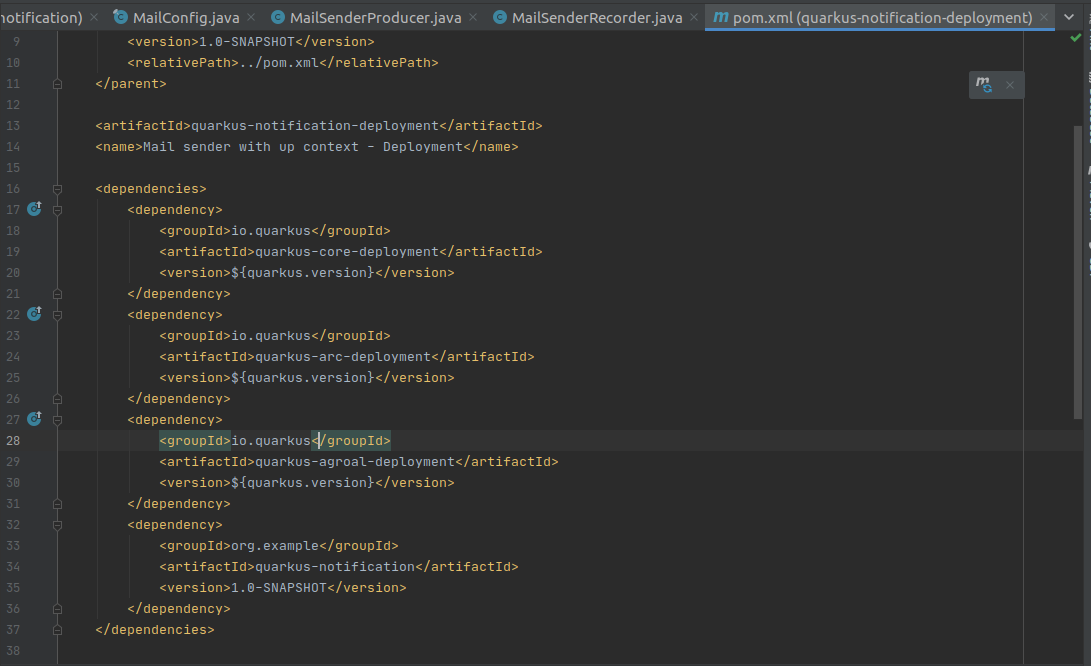
\includegraphics[width=\textwidth]{9}
\end{figure}

\subsection{Реализация Build Step Processors}
~

Как ранее упоминалось, buildStep это такая инструкция, которая позволяет пошагово настраивать бины и записивать их байткод через инструмент кваркус ARC.

	Теперь давайте реализуем три пошаговых процессора для записи байт-кода. 
Процессором первого шага сборки является метод feature(). Он отвечает за регистрацию расширения в ядро кваркуса.

	За второй шаг сборки отвечает метод build. Он отвечает за регистрацию необходимых BuildItem внутрь других BuildItem. Такой подход позволяет гибко настраивать бины. На этом этапе метод записывает байт-код для выполнения в статическом методе init. Мы настраиваем это через значение STATIC\_INIT, который указан в аннотации @Record.

	Третий шаг сборки описывает метод processSend. Данный метод записывает байт код, который будет выполняться в момент выполнения. Т.е. как только приложение запустится, сразу будет вызван метод отправки сообщения. 


\newpage
Код процессора выглядит следующим образом:

\begin{figure}[H]
	\centering
	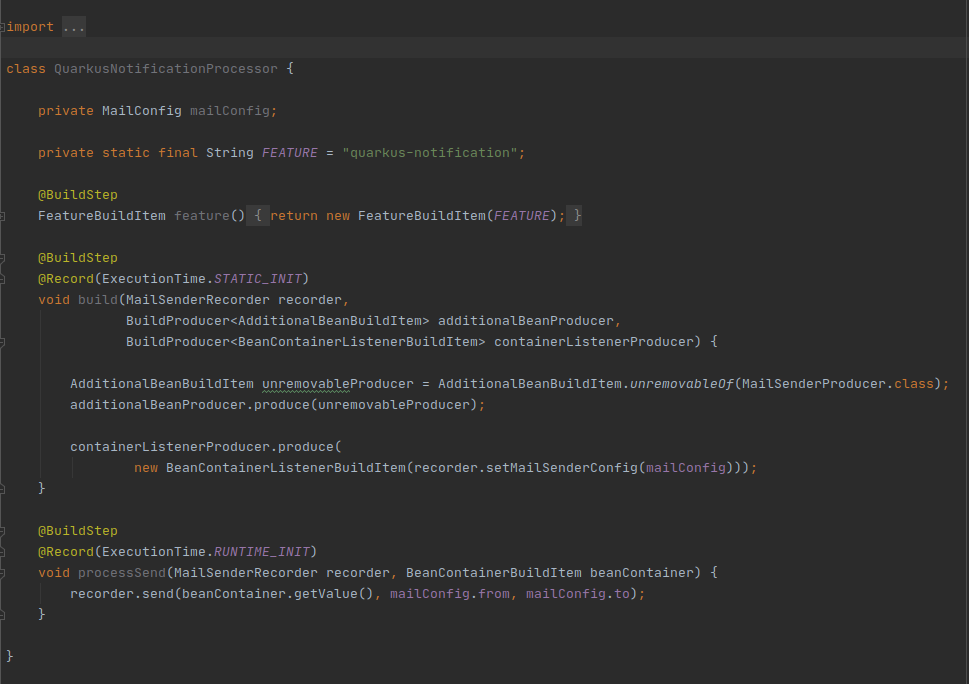
\includegraphics[width=\textwidth]{10}
\end{figure}

\newpage
\subsection{Тестирование}
~

Теперь можно протестировать работу расширения. Для этого подключаем ее как зависимость в наш новый проект. Для подключения нужно использовать группу и артефакт от модуля runtime.

\begin{figure}[H]
	\centering
	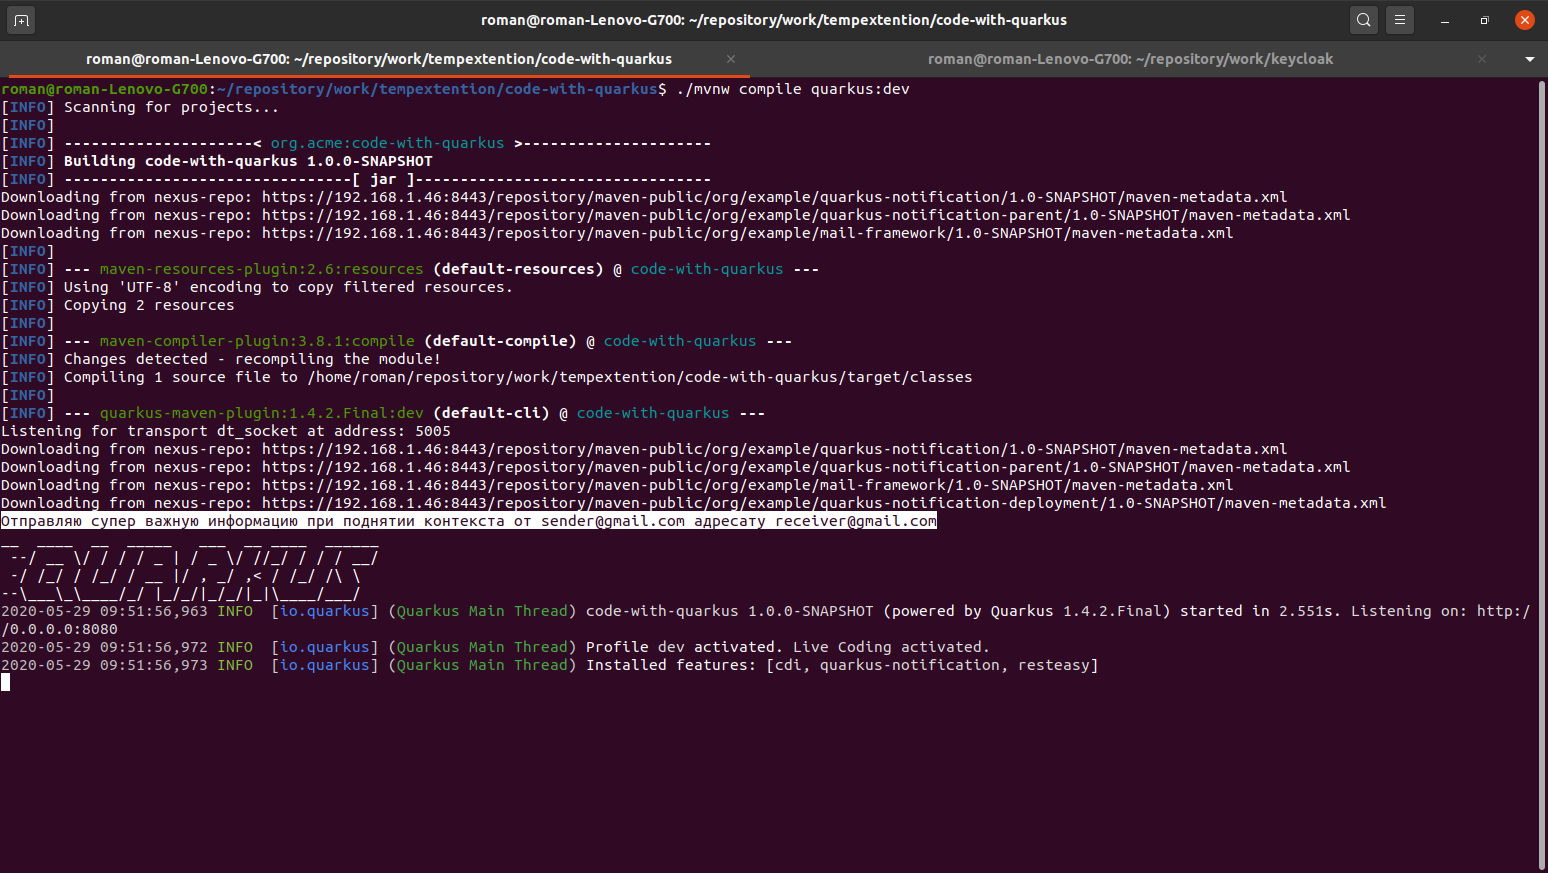
\includegraphics[width=\textwidth]{11}
\end{figure}
~

После запуска мы увидим, что отправляется наше импровизированное сообщение, а также увидим наше расширение в списке подключенных

\section{Пример реализации расширения на основе SPI}
~

Усложним прошлый пример тем, что пусть подключаемая библиотека предоставляет бины на основе SPI механизма. Что такое SPI? Service Provider Interface (SPI, Интерфейс поставщика услуг) это API, предназначенный для реализации или расширения третьей стороной. Его можно использовать для включения расширения каркаса и сменных компонентов. 
\newpage
\subsection{Структура нового сервиса}
~

Предположим, что вышла новая версия нашей импровизированной библиотеки. Теперь, она предоставляет бины посредством SPI и структура имеет следующий вид:

\begin{figure}[H]
	\centering
	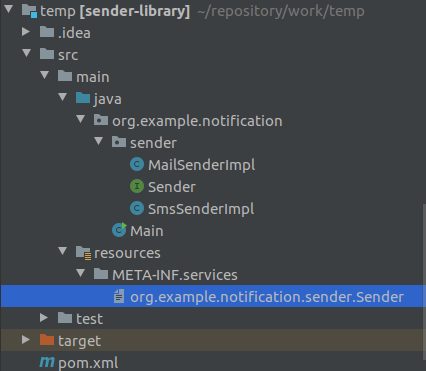
\includegraphics[width=\textwidth]{12}
\end{figure}

Структура в себе содержит простой интерфейс Sender, который предоставляет контракт по отправке сообщения, и две имплементации EmailSenderImpl и SmsSenderImpl. Первая имплементация подразумевает отправку сообщения через email, вторая через смс. 

Конкретный функционал будет упущен, для демонстрации будет пример, который будет печать в консоль эмуляцию отправки.

Разумеется, нужно взглянуть на SPI механизм. Предоставление расширений (бинов) происходит за счет регистрации конкретных реализации в файле org.example.notification.sender.Sender, который имеет такое название согласно своему имени класса.

\newpage
Содержимое этого файла имеет следующий вид:

\begin{figure}[H]
	\centering
	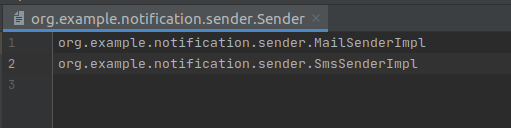
\includegraphics[width=\textwidth]{13}
\end{figure}

Как видно, тут зарегистрированны доступные реализации интерфейса Sender. Важно отметить, что количество реализаций может быть различным.

\subsection{Пишем расширения для SPI}
~

Расширение для этого примера, реализовано точно также, как и в пункте 4, но с новыми изменениями, которые никак не касаются структуры, направлены лишь на работу с SPI. Все изменения мы рассмотрим далее.
\subsubsection{Обзор runtime модуля}
~

Рантайм модуль состоит из двух классов. Структура кода представлена ниже:

\begin{figure}[H]
	\centering
	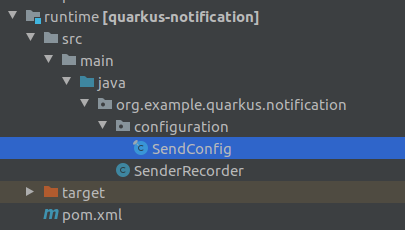
\includegraphics[width=15cm, height=8cm]{14}
\end{figure}

Первый класс SendConfig. 
Он отвечает за хранение значений в application.properties.
Второй, отвечает за верхнеуровневую работу по записи байт-кода. Код, который он может исполнять как во время статической инициализации, так и в рантайме. По сути, это форма отложенного выполнения, когда вызовы, сделанные во время развертывания, откладываются до времени выполнения. Отсюда и название.

Просмотр SendConfig опустим. Для ознакомления вы можете посмотреть исходный код в папке sources \textbf{(firs-extention-spi.zip)}.

Данный класс содержит 2 метода:
\begin{enumerate}
		\item[  1.] public List<Sender> registry(Collection<Class<? extends Sender>> implementationClasses)
		\item[  2.] public void sendAll(BeanContainer beanContainer, List<Sender> services, String from, String to)
\end{enumerate} 

Метод registry регистрирует бины, предварительно их создавая:

\begin{figure}[H]
	\centering
	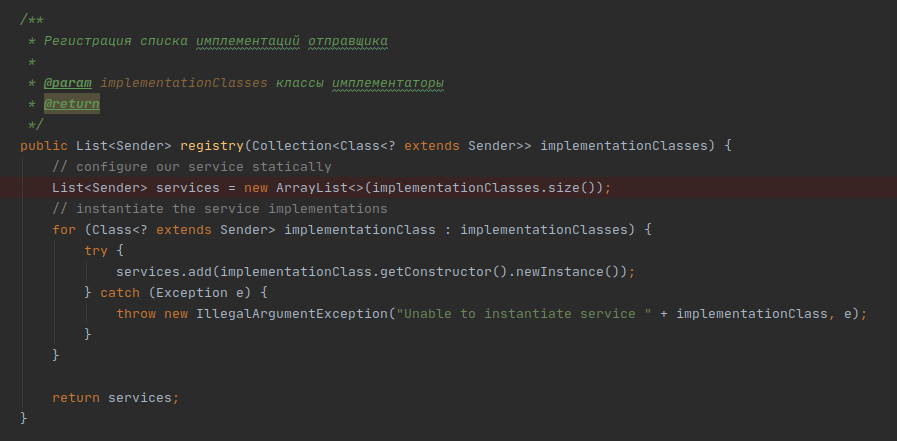
\includegraphics[width=\textwidth]{15}
\end{figure}
Второй метод sendAll, берет все имплементации и для каждой вызывает отправку.

\begin{figure}[H]
	\centering
	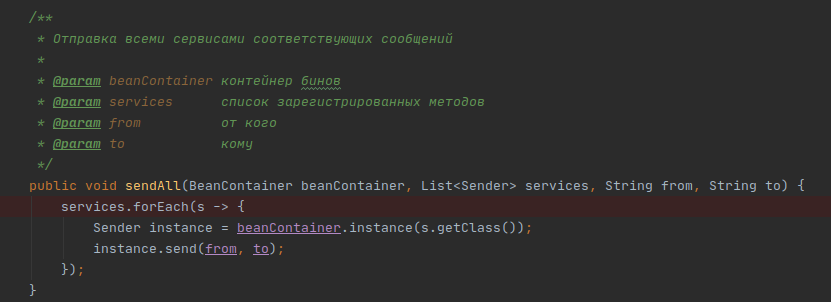
\includegraphics[width=\textwidth]{16}
\end{figure}

\newpage 
\subsubsection{Обзор deployment модуля}
~

Деплоймент модуль тоже претерпел маленьких изменений. Если для простого расширения, который практически ничего не делал не требовалось ничего, то сейчас можно увидеть, что структура немного поменялась и имеет вид:

\begin{figure}[H]
	\centering
	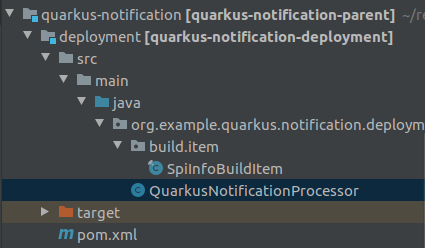
\includegraphics[width=\textwidth]{17}
\end{figure}

Как видим, структура почти не поменялась, оносительно предыдушего примера. SpiInfoBuildItem это новый класс, который необходимо для создания контекста при выполнении шагов сборки, которые помечены @BuildStep. 

Он имеет следующий вид:

\begin{figure}[H]
	\centering
	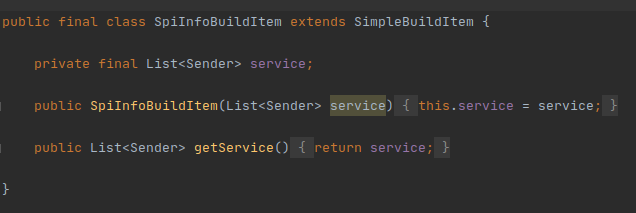
\includegraphics[width=\textwidth]{18}
\end{figure}

Что такое BuildItem? Это конкретные конечные подклассы абстрактного класса, предоставляемый самим кваркусом, io.quarkus.builder.item.BuildItem. Каждый элемент сборки представляет некоторую единицу информации, которая должна быть передана с одного этапа на другой. Базовый класс BuildItem не может быть непосредственно разделен на подклассы; скорее, существуют абстрактные подклассы для каждого из подклассов элементов сборки, которые могут быть созданы: простые, множественные и пустые.

Из содержания видно, что данная единица сборки предоставляет информацию о зарегистрированных сервисах. В данном случае он реализован для того, чтобы в момент регистрации он создавался, а в момент выполнения предоставлял зарегистрированные имплементации сервисов.

Рассмотрим процессор.

\subsubsection{Обзор процессора QuarkusNotificationProcessor}
~

Класс QuarkusNotificationProcessor содержит 3 метода, при этом являесть BuildStep-ом:
\begin{enumerate}
		\item[  1.] feature
		\item[  2.] registerNativeImageResources
		\item[  3.] processSend
\end{enumerate}

Часть из из них вам могут показаться уже знакомыми, т.к за основу был взят прошлый пример.

Метод feature мы пропустим, т.к. он генерируется автоматически при создании расширения. Стоит только отметить, что он нужен для того, чтобы зарегистрировать текущее расширение в ядре кваркуса.

Всю работу по регистрации внешних сервисов, которые нам поступают через SPI берет на себя метод registerNativeImageResources.Данный метод выглядит следующим образом:

\begin{figure}[H]
	\centering
	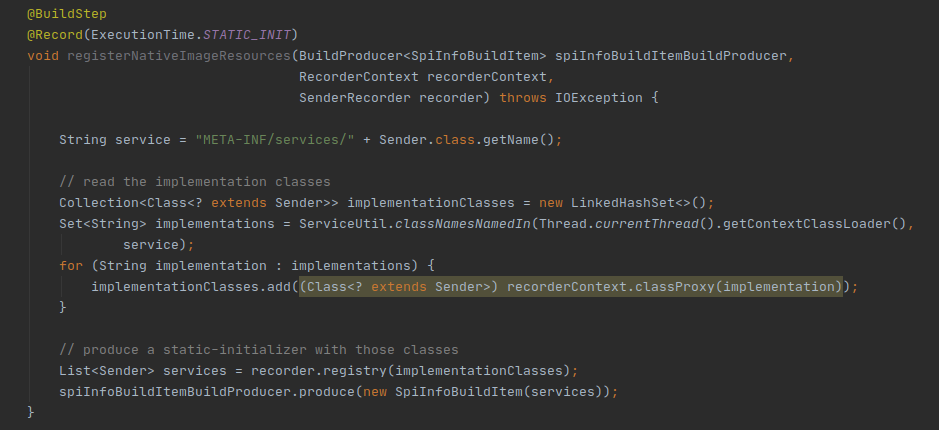
\includegraphics[width=\textwidth]{19}
\end{figure}

Если говорить коротко, то он собирает все описания из SPI файла (для простоты назовем его так), через рекордер создает для каждой имплементации соответствующий объект, а далее регистрируем наш SpiInfoBuildItem с этими сервисами. Как можно заметить, что все эти манипуляции будут происходить во время статической инициализации, т.е. в момент сборки расширения.

Метод processSend зарегистрирован в runtime фасе, т.е. как только будет запушено приложение, так сразу будет выполнен этот метод.

\newpage
Код метод очень простой:

\begin{figure}[H]
	\centering
	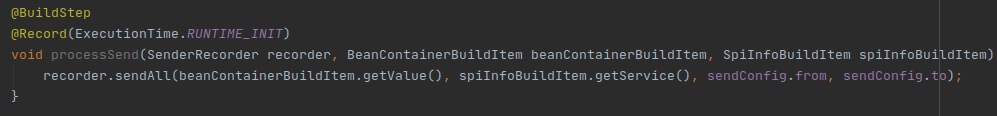
\includegraphics[width=\textwidth]{20}
\end{figure}

По коду видно, что в метод приходит наш SpiInfoBuildItem, который мы проинициализировали на этапе деплоя, и для всех этих сервисов будет сделан вызов отправки.

После того, как вы попробуете запустить приложение с нашим расширением, то вы столкнетесь с тем, что оно у вас упадет с ошибкой:

\begin{figure}[H]
	\centering
	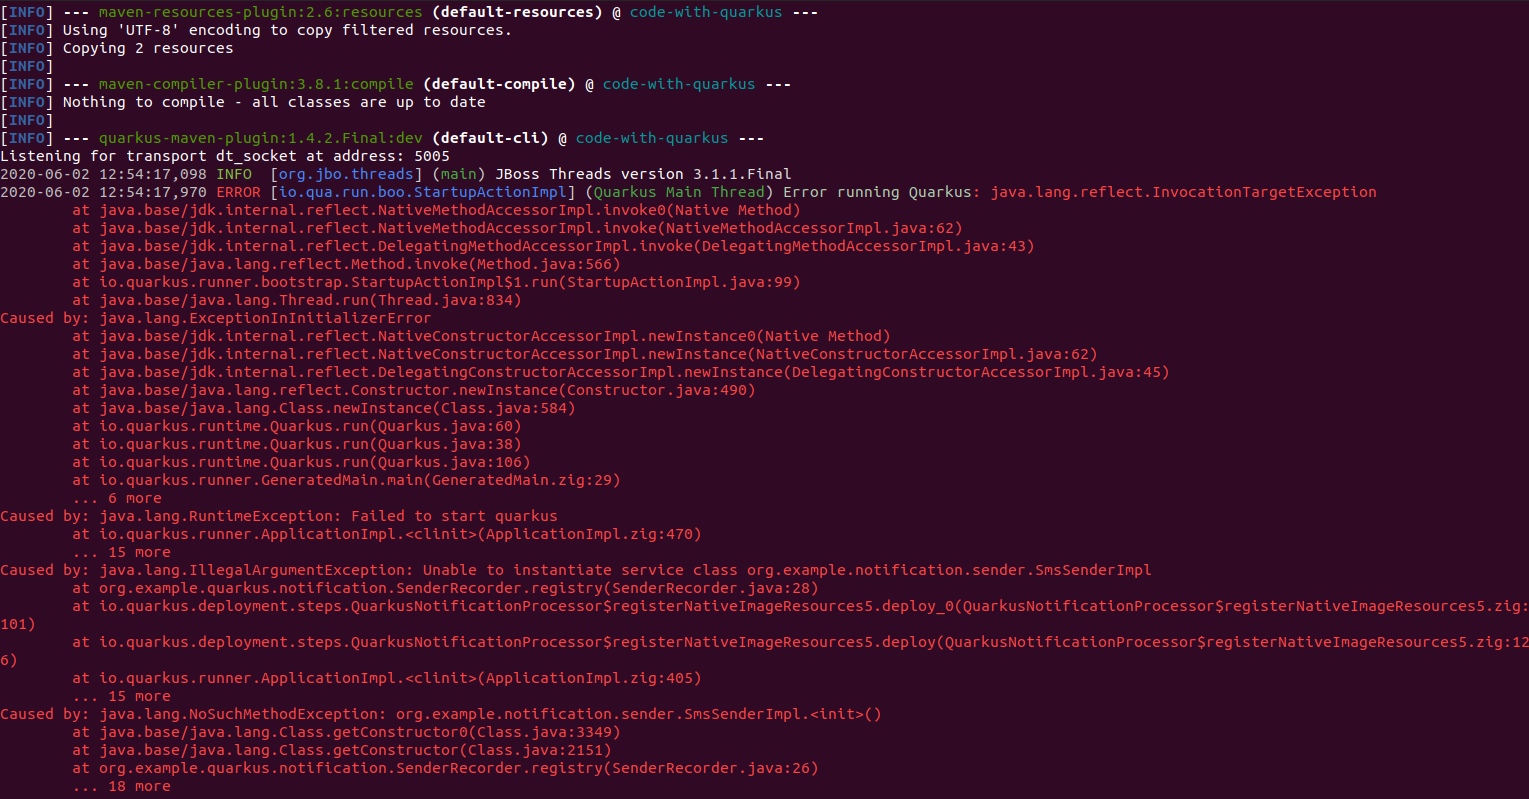
\includegraphics[width=\textwidth]{21}
\end{figure}

Это сделано специально. Изначально в одной из имплементаций интерфейса Sender я не создал конструктор по умолчанию. Это было сделано для того, чтобы показать, что библиотеки, могут содержать код, который вам нужен, но вы не можете его переписать сами. Для таких случаев необходимо использовать такое понятие, как "Подмена объектов" или Object Substitution.

\subsection{Подмена объектов (Object Substitution)}
~

Объекты, созданные на этапе сборки и переданные во время выполнения, должны иметь конструктор по умолчанию, чтобы их можно было создавать и настраивать при запуске среды выполнения из состояния времени сборки. Если у объекта нет конструктора по умолчанию, вы увидите ошибку.

Существует интерфейс io.quarkus.runtime.ObjectSubstitution, который можно реализовать, чтобы сообщить Quarkus, как обрабатывать такие классы. 

\newpage
Для этого необходимо создать в runtime модуле класс, который будет будет имплементировать данный интерфейс. В нашем случае пример такого класса можно видеть ниже:

\begin{figure}[H]
	\centering
	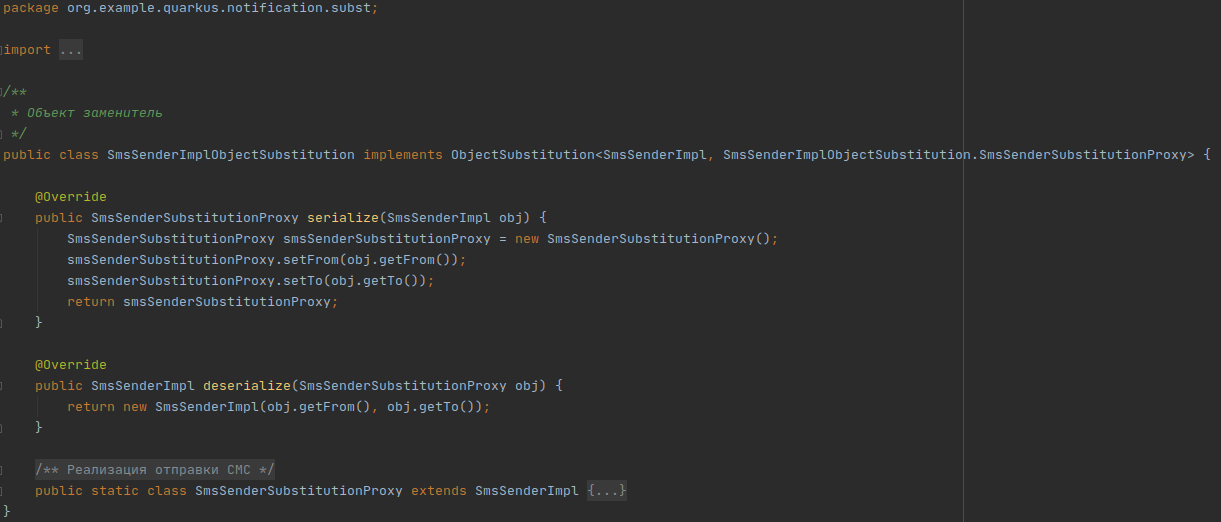
\includegraphics[width=\textwidth]{22}
\end{figure}

Интерфейс ObjectSubstitution принимает два типа. Первый, тип (SmsSenderImpl) нашего исходного класса, который в нашем случае не имеет конструктора по умолчанию. Второй, (SmsSenderImplObjectSubstitution.SmsSenderSubstitutionProxy) это класс заменитель, на который мы будем менять. Этот класс зарегистрирован прямо внутри SmsSenderImplObjectSubstitution - это не обязательное условие, вы также можете его создать отдельно.

Как видно, интерфейс ObjectSubstitution предоставляет два метода. Метод сериализации и десереализации. Именно эти методы отвечают за конвертацию одного объекта в другой без особых усилий со стороны разработчика. 
	Объект заместитель - это обычная имплементация, которая унаследована от искомого типа SmsSenderImpl:

\begin{figure}[H]
	\centering
	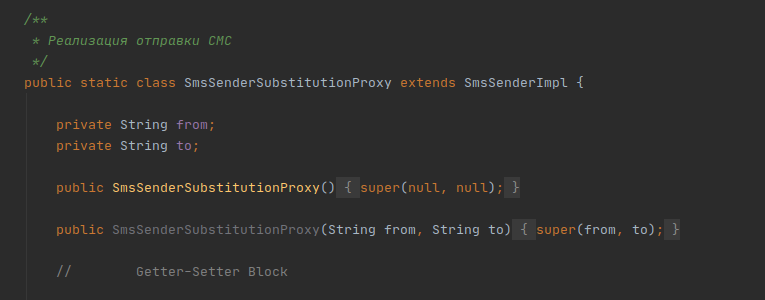
\includegraphics[width=\textwidth]{23}
\end{figure}

Все что нам необходимо, это просто создать конструктор по умолчанию, а методы оставить как есть. Нужно отметить, что работу методов тоже можно менять, но делать это стоит в зависимости от ваших требований.

\newpage
Кроме этого, нам нужно зарегистрировать эту замену в расширении. Для этого нужно добавить такой код в QuarkusNotificationProcessor:

\begin{figure}[H]
	\centering
	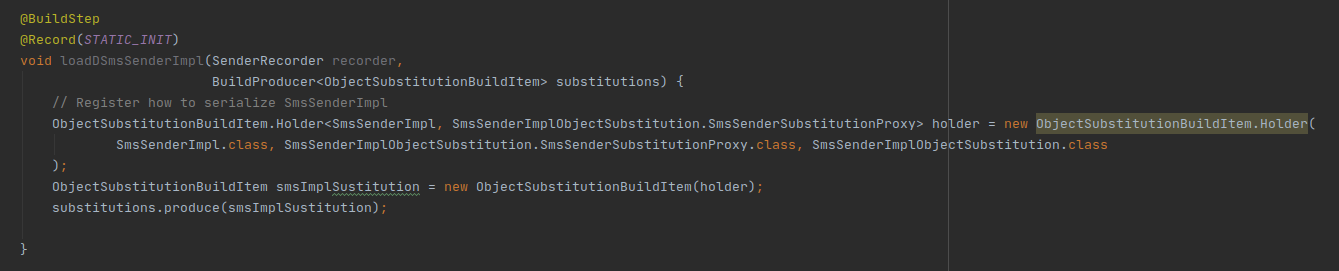
\includegraphics[width=\textwidth]{24}
\end{figure}

В методе происходит регистрация объекта заменителя, и с помощью специальной единицы сборки (ObjectSubstitutionBuildItem) мы предоставляем информацию для других сборок.

После того, как мы зарегистрируем эту единицу, само собой ничего не заработает, т.к. этим этапом сборки, мы всего лишь дали информацию кваркусу, о доступных единицах.

Последнее, что нужно сделать, это заменить нужный объект на объект прокси, для этого перейдем в функцию registerNativeImageResources и напишем следующий код: 

\begin{figure}[H]
	\centering
	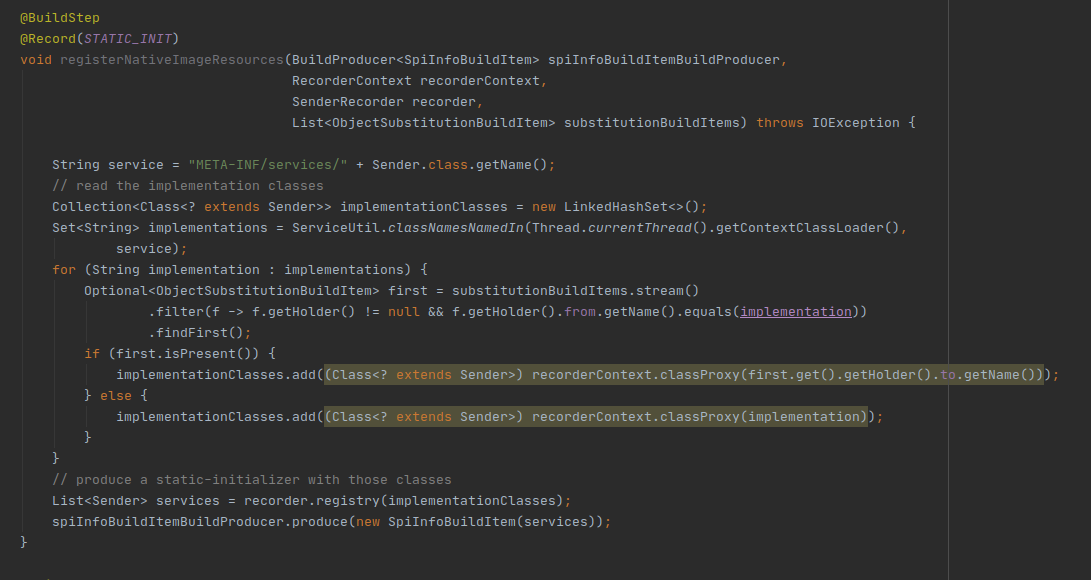
\includegraphics[width=\textwidth]{25}
\end{figure}

В месте, где мы добавляли имя настоящего класса, теперь мы добавляем имя прокси-класса, тем саммым решая проблему отсутствия конструктора по-умолчанию.

\newpage
\subsection{Тестирование расширения}

После того, как мы добавим расширение и запустим приложение, мы увидим следующие сообщения:

\begin{figure}[H]
	\centering
	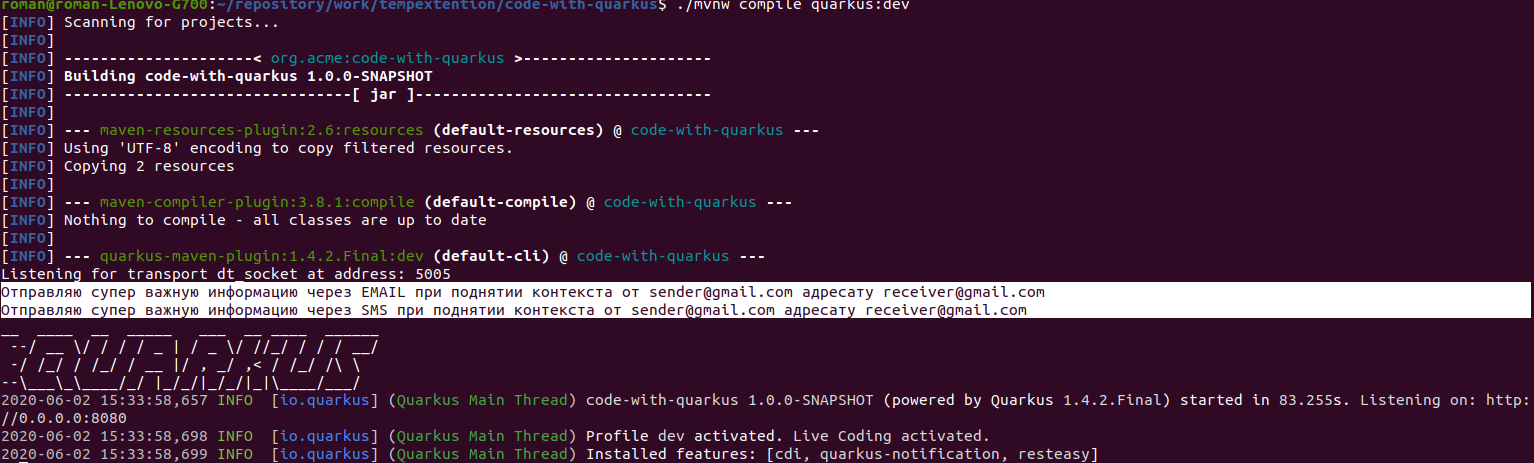
\includegraphics[width=\textwidth]{26}
\end{figure}

\subsection{Вывод}

Расширение Quarkus добавляет новое поведение, ориентированное на разработчиков, к основному приложению и состоят из двух отдельных частей: блоку сборки и блоку выполнения. Первая часть отвечает за всю сборку метаданных, такую как чтение аннотаций, XML-дескрипторы и т.д. Результатом этой фазы является записанный байт-код, который отвечает за непосредственное созданние соответствующих служб времени выполнения.

Это означает, что метаданные обрабатываются только один раз во время сборки, что экономит время запуска, а также использование памяти, поскольку классы и другие структуры, которые используются для обработки, не загружаются (или даже не присутствуют) в JVM времени выполнения.





\end{document}